\subsection{MSE Evaluation}
Finally we need to find a way of evaluating the model. The most common way is through the mean square error.
The MSE is given by 
\begin{equation}
MSE=\frac{1}{N}\sum_{1}^{N}{(Y_i-\hat{Y_i})}^2
\end{equation}
Where N is the number of samples, $Y$ is the vector containing the original undistorted values and $Y_hat$ is the predicted values.
\begin{lstlisting}
#CALCULATE MSE
y_hat=[[0]*Y.n for i in range(Y.m)]
Y=X*Coeff
for i in range(X.m):
y_hat[i][0]=get_point(BETA,X.matrix[i][0],X.matrix[i][1])
Y_hat=Matrix(y_hat)
Diff=Y_hat-Y
MSE=sum((Diff.peek(i,0)*Diff.peek(i,0)) for i in range(Diff.m))/Diff.m
\end{lstlisting}
Though the MSE doesn't give us a way of knowing how accurate the model is in general it is a great way for comparing models. The MSE could be used to compare this model to other models or even to change parameters in this model and how these changes affect the model's error.
\subsection{Graphical Evaluation}
Anoher way we can evaluate our model in the above specific scenarios is by comparing the generated graphs to the original graphs since we already know the original function. This is a good way to evaluate the model as it gives us a visual representation of how well the model is doing. We show below the original and predicted graphs for the single variable and multi-variable functions.
\begin{figure}[h!]
        
    \centering
    \begin{subfigure}{0.5\textwidth}
        \centering
        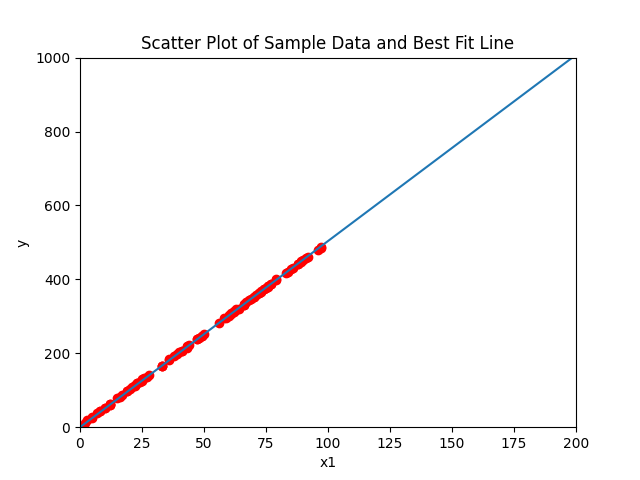
\includegraphics[scale=0.4]{One Variable Best Fit.png}
        \caption{Generated Best Fit Data}
    \end{subfigure}%
    \begin{subfigure}{0.5\textwidth}
        \centering
        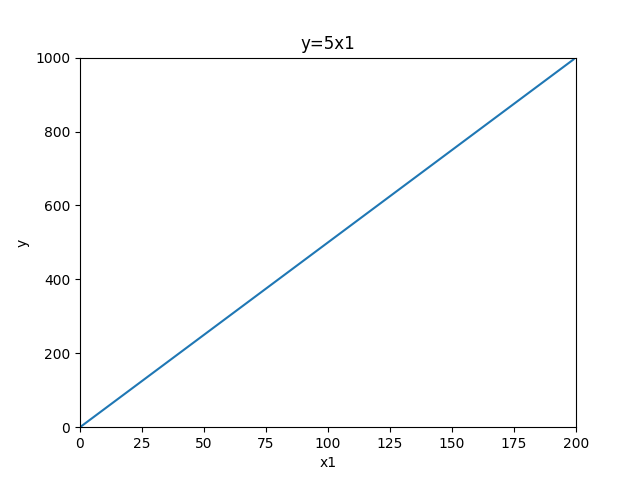
\includegraphics[scale=0.4]{One Variable Correct.png}
        \caption{Correct Best Fit Data}
    \end{subfigure}
    \caption{Comparison of Best Fit Data for Single Variable Linear Regression}
\end{figure}

\begin{figure}[!htb]
    \centering
    \begin{subfigure}{0.5\textwidth}
        \centering
        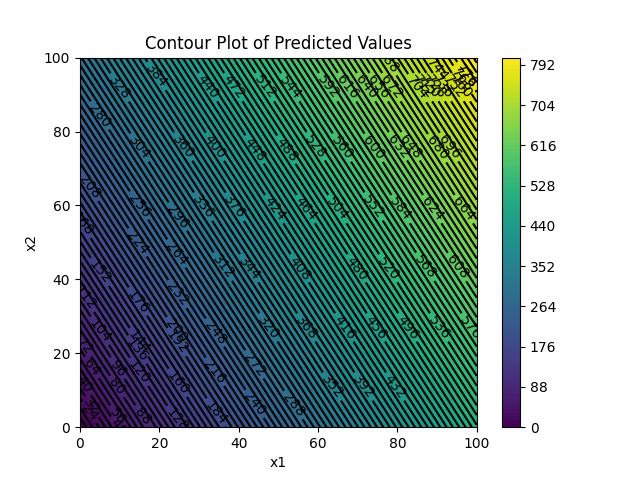
\includegraphics[scale=0.4]{Two Variable Predicted.png}
        \caption{Generated Best Fit Data}
    \end{subfigure}%
    \begin{subfigure}{0.5\textwidth}
        \centering
        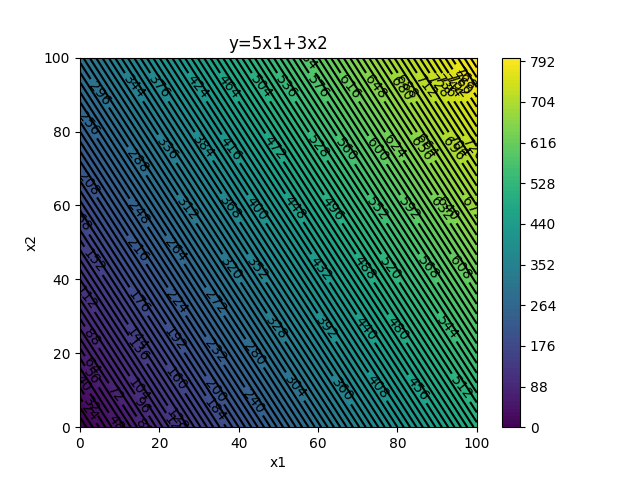
\includegraphics[scale=0.4]{Two Variable Corrected.png}
        \caption{Correct Best Fit Data}
    \end{subfigure}
    \caption{Comparison of Best Fit Data for Multivariable Linear Regression}
\end{figure}